\begin{exercise}
  Wir betrachten das zweidimensionale Poisson Problem mit homogenen
  Dirichlet-Randbedingungen, siehe $(7.19)$ des Vorlesungsskriptes. Geben Sie
  die Diskretisierungsmatrix $A_h$ und die rechte Seite $g_h$ des entstehenden
  linearen Gleichungssystems an, wenn dieses Problem mit Finiten Differenzen der
  Schrittweite $h_1 = h_2 = h > 0$ diskretisiert wird. Beginnen Sie der Einfachheit
  halber mit dem Gitter aus Abb. 1. Dazu sollten Sie die Unbekannten
  $y_{j,k} \approx y(x_{j,k})$ wie folgt ordnen

  \begin{align}\label{sec}
    y_{1,1}, \dots , y_{N_2 -1}, \text{ }
    y_{2,1}, \dots , y_{2,N_2 -1} \text{ }
    y_{3,1}, \dots
  \end{align}
  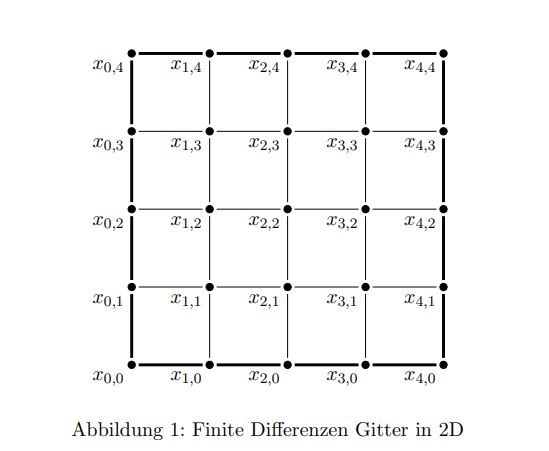
\includegraphics{Abbildung_1}
  \end{exercise}

\begin{solution}
  Beweis.
\end{solution}
